\section{Elementary Ring Theory}

See 肖梁

In this course, all rings are assumed to be unital and $1 \neq 0$.

\begin{figure}[H]
\centering
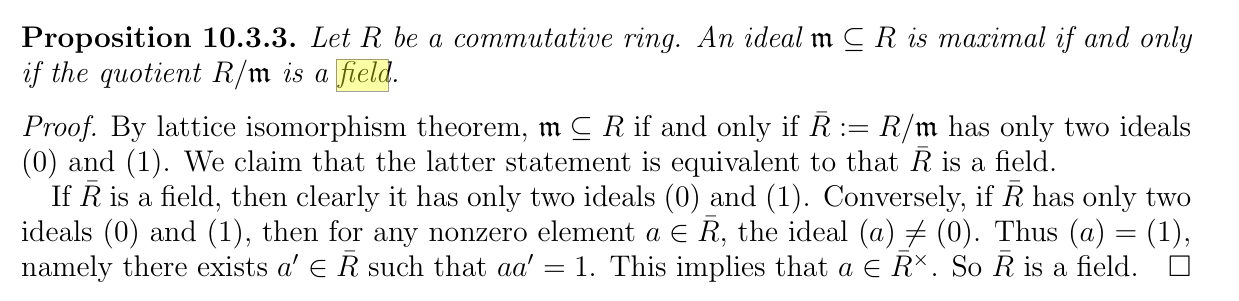
\includegraphics[width=\textwidth]{1-elementary-ring-theory-2025050816.png}
% \caption{}
\label{}
\end{figure}

\begin{note}
Field only has zero ideal.
\end{note}
If $I$ is an ideal such that $M\subset I\subset S$ then $(0)\subset I/M\subset S/M$, $I/M$ is an ideal of the field $S/M$ thus is zero. Therefore, $M$ is maximal.

\begin{exercise}
Let $R$ be a commutative ring. If all submodules of finitely generated free modules over $R$ are free over $R$, then $R$ is a PID.
\end{exercise}
\begin{definition}[\textbf{Finitely generated free module over $R$}]
A module $M$ over a ring $R$ is called a \textbf{finitely generated free module} if it has a basis consisting of a finite number of elements.
This means there exists a finite set of elements $\{b_1, \ldots, b_n\} \subset M$ such that every element $m \in M$ can be written uniquely in the form
\[
m = r_1 b_1 + r_2 b_2 + \cdots + r_n b_n
\]for some unique coefficients $r_1, \ldots, r_n \in R$.
Such a module is isomorphic to the direct sum of $n$ copies of $R$, denoted $R^n$.
\end{definition}
\begin{note}
The definition of $M$ as $R$ -module  is similar to $V$ as $K$ -linear space.
\end{note}
\begin{definition}[free $R$-module]
An $R$-module $F$ is a \textbf{free $R$-module} if it has a basis, i.e., there exists a subset $B \subseteq F$ such that for every $x \in F$, there is a unique finite subset $\{b_1, \ldots, b_n\} \subseteq B$ and unique scalars $\{r_1, \ldots, r_n\} \subseteq R$ such that $x = r_1 b_1 + \cdots + r_n b_n$. Equivalently, $F$ is isomorphic to a direct sum of copies of $R$, denoted $R^{(I)}$ for some index set $I$.
\end{definition}
\subsection{Problem 1}

\begin{theorem}
Let $R$ be a commutative ring. If all submodules of finitely generated free modules over $R$ are free over $R$, then $R$ is a PID.
\end{theorem}
\begin{proof}
First prove that $R$ is an \underline{integral domain}. Suppose that $a, b \in R \backslash\{0\}$ with $a b=0$. Consider $a R \subseteq R$; it is a submodule of free module; so $a R$ is a free $R$-module. However, we know that $b$ kills all of $a R$ because $a b=0$; this contradicts that $a R$ is a free $R$-module.

Let $I \subseteq R$ be an ideal; it is then a free $R$-submodule of $R$. We claim that $I$ is a free module of rank 1 over $R$. Suppose not, then there exist $\left(\alpha_j\right)_{j \in J}$ forming an $R$-basis of $I$. But if $\# J \geq 2$, we know that $\alpha_j \cdot\left(\alpha_i\right)+\alpha_i \cdot\left(-\alpha_j\right)=0$, contradiction! This says that $I$ is free of rank one, i.e. $I$ is generated by one element $\alpha \in I$ so that $I=(\alpha)$ is a principal ideal. Thus $R$ is a PID.
\end{proof}

\subsubsection{Explanation}

Okay, let's break down this proof step by step.

\textbf{The Statement to be Proven:}

"Let $R$ be a commutative ring. If all submodules of finitely generated free modules over $R$ are free over $R$, then $R$ is a PID."

Let's define the key terms:

\begin{itemize}
	\item \textbf{Commutative Ring ($R$)}: A set with addition and multiplication operations that satisfy certain properties (associativity, commutativity of both operations, distributivity, additive identity 0, additive inverses, multiplicative identity 1). "Commutative" means $ab = ba$ for all $a,b \in R$.
	\item \textbf{Module over $R$ (or $R$ -module)}: Similar to a vector space over a field, but scalars come from a ring $R$.
	\item \textbf{Free $R$ -module}: An $R$ -module that has a basis, i.e., a linearly independent spanning set. A finitely generated free module has a finite basis. $R$ itself is a free $R$ -module of rank 1 (with basis $\{1\}$). $R^n$ (tuples of $n$ elements from $R$) is a free $R$ -module of rank $n$.
	\item \textbf{Submodule}: A subset of a module that is itself a module under the same operations and with scalars from the same ring.
	\item \textbf{PID (Principal Ideal Domain)}: An integral domain in which every ideal is principal.
	\begin{itemize}
		\item \textbf{Integral Domain}: A commutative ring with no zero divisors (if $a,b \in R$ and $ab=0$, then either $a=0$ or $b=0$).
		\item \textbf{Ideal}: A submodule of $R$ (when $R$ is considered as a module over itself). More formally, a subset $I \subseteq R$ such that $(I,+)$ is a subgroup of $(R,+)$, and for any $r \in R$ and $x \in I$, $rx \in I$.
		\item \textbf{Principal Ideal}: An ideal generated by a single element, i.e., an ideal of the form $I = (a) = \{ra \mid r \in R\}$ for some $a \in R$.
	\end{itemize}
\end{itemize}

\textbf{The Hypothesis:} All submodules of finitely generated free modules over $R$ are free over $R$.

\textbf{The Goal:} Prove that $R$ is a PID. This requires proving two things:

\begin{enumerate}
	\item $R$ is an integral domain.
	\item Every ideal in $R$ is principal.
\end{enumerate}


\textbf{Proof Breakdown:}

\textbf{Part 1: Prove that $R$ is an integral domain.}

\begin{itemize}
	\item \textbf{"Suppose that $a, b \in R \backslash\{0\}$ with $a b=0$."}
This is the standard way to start a proof that $R$ is an integral domain by contradiction. We assume $R$ is \textit{not} an integral domain, which means there exist non-zero elements $a$ and $b$ whose product is zero. Our goal is to show this assumption leads to a contradiction, forcing us to conclude that such $a$ and $b$ cannot exist (meaning if $ab=0$, then $a=0$ or $b=0$).
	\item \textbf{"Consider $a R \subseteq R$; it is a submodule of free module; so $a R$ is a free $R$ -module."}
	\begin{itemize}
		\item $R$ itself can be considered as a (finitely generated) free $R$ -module of rank 1 (its basis is just the element $\{1\}$).
		\item $aR$ is the set $\{ar \mid r \in R\}$. This is an ideal in $R$, and every ideal is a submodule of $R$ (when $R$ is viewed as an $R$ -module).
		\item Since $R$ is a finitely generated free module, and $aR$ is a submodule of $R$, the hypothesis of the theorem applies: "$aR$ is a free $R$ -module."
	\end{itemize}
	\item \textbf{"However, we know that $b$ kills all of $a R$ because $a b=0$; this contradicts that $a R$ is a free $R$ -module."}
	\begin{itemize}
		\item "Kills" means $b \cdot x = 0$ for all $x \in aR$. Let $x \in aR$. Then $x = ar_0$ for some $r_0 \in R$.
		\item So, $b \cdot x = b(ar_0) = (ba)r_0$. Since we assumed $ab=0$ (and $R$ is commutative, so $ba=0$), we have $(ba)r_0 = 0 \cdot r_0 = 0$.
		\item So, $b \cdot x = 0$ for all $x \in aR$.
		\item Now, why is this a contradiction to $aR$ being a free $R$ -module?
		\begin{itemize}
			\item If $aR$ is a free $R$ -module, it has a basis.
			\item Case 1: $aR = \{0\}$ (the zero module). This means $a \cdot 1 = a = 0$. But we started by assuming $a \in R \backslash\{0\}$ (i.e., $a \neq 0$). So this case is ruled out by our initial assumption about $a$.
			\item Case 2: $aR \neq \{0\}$. Then $aR$ is a non-zero free $R$ -module. Let $\{e_k\}_{k \in K}$ be a basis for $aR$. Since $aR \neq \{0\}$, there is at least one basis element, say $e_1 \neq 0$.
			\item Since $e_1 \in aR$, we know from above that $b \cdot e_1 = 0$.
			\item If an element $b \neq 0$ annihilates a non-zero element $e_1$ in a free module, this means that the module cannot be free \textit{unless} $b$ forces all coefficients to be zero in some sense.
			\item More precisely: A free module $M$ over a ring $R$ has the property that if $r \cdot m = 0$ for some $r \in R$ and $m \in M$, then either $r$ is a zero divisor for elements related to $m$, or $m=0$. If $M$ is free with basis $\{e_k\}$, then any $m \in M$ can be written as $m = \sum c_k e_k$. If $r \cdot m = \sum r c_k e_k = 0$, then by linear independence, $r c_k = 0$ for all $k$.
			\item Here, $aR$ is free. If $aR \neq \{0\}$, it has a non-empty basis, say $\{\beta_j\}_{j \in J}$. Take any basis element $\beta_j$. We know $b \cdot \beta_j = 0$. Since $\beta_j \neq 0$ (it's a basis element of a non-zero module) and $b \neq 0$ (by assumption), this implies that $b$ is a zero-divisor "acting on" $\beta_j$.
			\item The crucial property of a free module $M$ over a ring $R$ is that if $r \in R$ annihilates \textit{every} element of $M$ (i.e., $r \cdot m = 0$ for all $m \in M$), and $M \neq \{0\}$, then $r$ must be $0$.
			\item In our situation, $b \neq 0$ and $aR \neq \{0\}$ (since $a \neq 0$). We have $b \cdot x = 0$ for all $x \in aR$. This means $b$ is a non-zero element that annihilates the entire non-zero module $aR$. This can only happen if $aR$ is not actually free (unless $R$ itself has issues). The only way a non-zero scalar can annihilate every element of a non-zero free module is if the module itself is the zero module (which we've ruled out because $a \neq 0$) or if the ring itself isn't "nice."
			\item \textbf{The more direct contradiction:} A non-zero free module cannot have a non-zero annihilator. The set of elements $r \in R$ such that $r \cdot m = 0$ for all $m \in M$ is called the annihilator of $M$, denoted $\text{Ann}_R(M)$. If $M$ is a free $R$ -module and $M \neq \{0\}$, then $\text{Ann}_R(M) = \{0\}$.
Here, $M = aR$. Since $a \neq 0$, $aR \neq \{0\}$ (as $a \cdot 1 = a \in aR$). We found that $b \in \text{Ann}_R(aR)$. But we assumed $b \neq 0$. This means $\text{Ann}_R(aR) \neq \{0\}$, which contradicts the fact that $aR$ is a non-zero free module.
		\end{itemize}
	\end{itemize}
	\item This contradiction shows that our initial assumption ($a, b \in R \backslash\{0\}$ with $ab=0$) must be false. Therefore, $R$ must be an integral domain.
\end{itemize}

\textbf{Part 2: Let $I \subseteq R$ be an ideal; it is then a free $R$ -submodule of $R$. We claim that $I$ is a free module of rank 1 over $R$.}

\begin{itemize}
	\item \textbf{"Let $I \subseteq R$ be an ideal; it is then a free $R$ -submodule of $R$."}
	\begin{itemize}
		\item An ideal $I$ of $R$ is, by definition, a submodule of $R$ (when $R$ is considered as an $R$ -module).
		\item As established before, $R$ is a finitely generated free $R$ -module (rank 1, basis $\{1\}$).
		\item By the hypothesis of the theorem, any submodule of a finitely generated free module is free. Thus, $I$ must be a free $R$ -module.
	\end{itemize}
	\item \textbf{"We claim that $I$ is a free module of rank 1 over $R$."}
This means $I$ should have a basis consisting of a single element. If $I = (\alpha)$ for some $\alpha \in I$, then $\{\alpha\}$ would be its basis (assuming $\alpha \neq 0$).
	\item \textbf{"Suppose not, then there exist $\left(\alpha_j\right)_{j \in J}$ forming an $R$ -basis of $I$. But if $\# J \geq 2$, we know that $\alpha_j \cdot\left(\alpha_i\right)+\alpha_i \cdot\left(-\alpha_j\right)=0$, contradiction!"}
	\begin{itemize}
		\item Let's assume the rank of $I$ (as a free $R$ -module) is not 1.
		\begin{itemize}
			\item Could the rank be 0? If rank is 0, $I = \{0\}$, which is the principal ideal $(0)$. This fits the "rank 1 or 0" pattern, as $(0)$ is generated by one element. So the argument is primarily against rank $\ge 2$.
			\item So, assume the rank is greater than or equal to 2. This means there are at least two distinct basis elements in any basis for $I$. Let $\alpha_i$ and $\alpha_j$ be two distinct elements from such a basis.
		\end{itemize}
		\item Consider the expression: $\alpha_j \cdot (\alpha_i) + \alpha_i \cdot (-\alpha_j)$.
		\begin{itemize}
			\item Here, $\alpha_i$ and $\alpha_j$ are elements of the ideal $I$, and also elements of the ring $R$.
			\item The coefficients are $(\alpha_j)$ and $(-\alpha_j)$, which are also elements of $R$.
			\item The expression is a linear combination of the basis elements $\alpha_i$ and $\alpha_j$.
			\item $\alpha_j \cdot \alpha_i + \alpha_i \cdot (-\alpha_j) = \alpha_j \alpha_i - \alpha_i \alpha_j$.
			\item Since $R$ is a commutative ring (this was stated at the beginning), $\alpha_j \alpha_i = \alpha_i \alpha_j$.
			\item So, $\alpha_j \alpha_i - \alpha_i \alpha_j = 0$.
		\end{itemize}
		\item This is a linear combination of basis elements that equals zero:
$c_1 \alpha_i + c_2 \alpha_j = 0$, where $c_1 = \alpha_j$ and $c_2 = -\alpha_j$.
		\item For a set of elements to be a basis, they must be linearly independent. This means if a linear combination of them is zero, all coefficients must be zero.
		\item So, we must have $c_1 = \alpha_j = 0$ and $c_2 = -\alpha_j = 0$.
		\item But if $\alpha_j = 0$, then it cannot be a basis element of a free module (unless the module is the zero module, which would have an empty basis or rank 0, not $\ge 2$). Basis elements are non-zero.
		\item \textbf{The contradiction:} We found a linear combination of distinct basis elements $\alpha_i, \alpha_j$ which is $\alpha_j (\alpha_i) + (-\alpha_i) (\alpha_j) = 0$. For this to not violate linear independence, the coefficients must be zero. That is, $\alpha_j=0$ and $-\alpha_i=0$. But basis elements of a free module must be non-zero if the module itself is non-zero (and if $I$ has rank $\ge 2$, it's non-zero).
		\item This specific relation $\alpha_j (\alpha_i) - \alpha_i (\alpha_j) = 0$ is always true in a commutative ring. If $\alpha_i, \alpha_j$ are part of a basis for an ideal $I \subseteq R$, and these are considered as elements of the module $I$, the coefficients in the linear combination are $\alpha_j \in R$ and $-\alpha_i \in R$.
		\item If $I$ is non-zero, and its basis has at least two elements $\alpha_1, \alpha_2$. Then $\alpha_2 \cdot \alpha_1 + (-\alpha_1) \cdot \alpha_2 = 0$.
		\item For this to be a non-trivial relation, at least one of the coefficients $\alpha_2$ or $-\alpha_1$ must be non-zero. Since $\alpha_1, \alpha_2$ are basis elements, they are non-zero (assuming $I \neq (0)$). So the coefficients $\alpha_2$ and $-\alpha_1$ are non-zero (since $R$ is now an integral domain, if $-\alpha_1 = 0$, then $\alpha_1=0$, which is not possible for a basis element).
		\item So we have a linear combination of basis elements equal to zero, where the coefficients are non-zero elements from $R$. This contradicts the definition of a basis for a free module over an integral domain $R$ (unless $R$ was the zero ring, which it isn't as it has a 1 and is an integral domain).
		\item Therefore, the assumption that the rank of $I$ is $\geq 2$ must be false.
	\end{itemize}
	\item \textbf{"This says that $I$ is free of rank one, i.e. $I$ is generated by one element $\alpha \in I$ so that $I=(\alpha)$ is a principal ideal."}
	\begin{itemize}
		\item Since $I$ is a free $R$ -module and its rank cannot be $\geq 2$, its rank must be 0 or 1.
		\begin{itemize}
			\item If rank is 0, then $I=\{0\}$, which is the principal ideal $(0)$.
			\item If rank is 1, then $I$ has a basis consisting of a single element, say $\{\alpha\}$, where $\alpha \in I$. This means every element $x \in I$ can be written uniquely as $x = r \cdot \alpha$ for some $r \in R$. This is precisely the definition of the principal ideal generated by $\alpha$, i.e., $I = (\alpha)$.
		\end{itemize}
		\item So, every ideal $I$ in $R$ is a principal ideal.
	\end{itemize}
\end{itemize}

\textbf{Conclusion:}

\begin{itemize}
	\item We have shown that $R$ is an integral domain (Part 1).
	\item We have shown that every ideal $I$ in $R$ is a principal ideal (Part 2).
\end{itemize}

By definition, an integral domain in which every ideal is principal is a \textbf{Principal Ideal Domain (PID)}.
Thus, the proof is complete.

\subsection{Problem 2}

\begin{exercise}
Let $k$ be a finite field with $q$ elements.
	\begin{enumerate}
		\item How many monic irreducible polynomials are there in $k[x]$ of each degree $d=2,3,4,5,6$?
		\item What are the possible Galois groups of the splitting field of a (not necessarily irreducible) polynomial of degree 5 over $k$? Why?
	\end{enumerate}
\end{exercise}
\begin{proof}
(1) Each irreducible polynomial of degree 2 has exactly two zeros in $\mathbb{F}_{q^2}-\mathbb{F}_q$.

\begin{note}
Denote one zero of the irreducible polynomial $f(x)$ by $\alpha,\beta$, then $\alpha \not\in \mathbb{F}_{q}$, otherwise $\alpha\in \mathbb{F}_{q}\Rightarrow\beta\in \mathbb{F}_{q}$, thus $f (x)\in \mathbb{F}_{q}[x]$, which is a contradiction.
Claim that $\alpha\in \mathbb{F}_{q^2}$. Since $m_{\alpha,\mathbb{F}_{q}}(x)|f(x)$, $\alpha \not\in \mathbb{F}_{q}$, then $x-\alpha \not\in \mathbb{F}_{q}[x]$, $\deg m_{\alpha,\mathbb{F}_{q}}(x)\geq2$; but $\deg m_{\alpha,\mathbb{F}_{q}}(x)\leq \deg f(x)=2$ and the minimal polynomial of $\alpha$ is unique (by definition); so $m_{\alpha,\mathbb{F}_{q}}(x)=f(x)$. $\mathbb{F}_{q}(\alpha)$ is the spliting field of $f(x)$ over $\mathbb{F}_{q}$, with degree $2$. $[\mathbb{F}_{q}(\alpha),\mathbb{F}_{q}]=2$, which means $\mathbb{F}_{q}(\alpha)$ is a 2-dimensional vector space over $\mathbb{F}_{q}$; $\mathbb{F}_{q}(\alpha)=\mathbb{F}_{q}\oplus \mathbb{F}_{q}$, thus $\lvert \mathbb{F}_{q}(\alpha) \rvert=q^2$.
Claim that $\mathbb{F}_{q}(\alpha)\cong \mathbb{F}_{q^2}$. This refers to the construction of $\mathbb{F}_{q^2}$, more generally, $\mathbb{F}_{q^n}$, which is the splitting field of $x^{q^{n}}-x$ over $\mathbb{F}_{q}$. It suffices to verify that every field with $q^2$ elements is a\footnote{"a" means "the", since the splitting field is unique up to isomorphism.} splitting field of $x^{q^{2}}-x$ over $\mathbb{F}_{q}$. Consider the multiplitcative group, $\mathbb{F}_{q}(\alpha)^{\times}$; it has $q^2-1$ elements. For any $a\in \mathbb{F}_{q}(\alpha)^{\times}$, by Lagrange's theorem from group theory, $q^2-1=\lvert \mathbb{F}_{q}(\alpha)^{\times} \rvert=[\mathbb{F}_{q}(\alpha)^{\times}:a]\cdot \lvert \left< a \right> \rvert$ is divided by $\lvert a \rvert$, the order of $a$; thus $a^{q^2-1}=1$; $a$ is the solution of $x^{q^2-1}-1=0$. Including $0$, then any element in $\mathbb{F}_{q}(\alpha)$ is the solution of $x^{q^2}-x=0$, which has $q^2$ distinct zeros. Since $\mathbb{F}_{q}(\alpha)$ also has $q^2$ distinct elements, they correspond to $q^2$ different roots of $x^{q^2}-x=0$. By the definition of $\mathbb{F}_{q^2}$, $\mathbb{F}_{q}(\alpha)\cong \mathbb{F}_{q^2}$; thus $\alpha\in \mathbb{F}_{q^2}$; similarly, $\beta\in \mathbb{F}_{q^2}$.
\end{note}
So there are $\frac{q^2-q}{2}$ irreducible polynomials of degree 2.

\begin{note}
This is because, every element in the extension of $\mathbb{F}_{q}$ has a \underline{unique} minimal polynomial $m_{\alpha,\mathbb{F}_{q}}(x)$, which is the definition of minimal polynimial. We know that $f(x)$ is the minimal polynomial of exactly two elements, $\alpha,\beta$ in $\mathbb{F}_{q^2}-\mathbb{F}_{q}$; each irreducible polynomial of degree 2 corresponds to 2 different elements in $\mathbb{F}_{q^2}-\mathbb{F}_{q}$. Thus there are $\frac{q^2-q}{2}$ irreducible polynomials of degree 2. We are done!
\end{note}
Similarly, there are $\frac{q^3-q}{3}$ irreducible polynomials of degree 3, and there are $\frac{q^5-q}{5}$ irreducible polynomials of degree 5.

Each irreducible polynomial of degree 4 corresponds to four elements of $\mathbb{F}_{q^4}-\mathbb{F}_{q^2}$; so there are $\frac{q^4-q^2}{4}$ irreducible polynomials of degree 4.

Each irreducible polynomial of degree 6 corresponds to six elements of $\mathbb{F}_{q^6}-(\mathbb{F}_{q^2} \cup \mathbb{F}_{q^3})$; there are $\frac{q^6-q^3-q^2+q}{6}$ such polynomials.

\begin{note}
We know that
\[
\lvert \mathbb{F}_{q^2}\cup \mathbb{F}_{q^{3}} \rvert=\lvert \mathbb{F}_{q^2} \rvert+\lvert \mathbb{F}_{q^3} \rvert-\lvert \underbrace{ \mathbb{F}_{q^2}\cap \mathbb{F}_{q^{3}} }_{ =\mathbb{F}_{q} } \rvert=q^2+q^{3}-q
\]
\end{note}
(2) The factorization of $f$ into irreducibles corresponds to partitions of 5:

If $f$ is irreducible, the splitting field is $\mathbb{F}_{q^5}$. The associated Galois group is $Z_5$.

If $f$ factors as the product of a degree 2 and a degree 3 polynomials, the splitting field is $\mathbb{F}_{q^6}$. The associated Galois group is $Z_6$.

In other cases, we can get similarly $\mathbb{F}_{q^4}, \mathbb{F}_{q^3}, \mathbb{F}_{q^2}$, and $\mathbb{F}_q$. The associated Galois groups are $Z_4, Z_3, Z_2, \{1\}$, respectively.
\end{proof}

\subsection{A UFD property}

\begin{figure}[H]
\centering
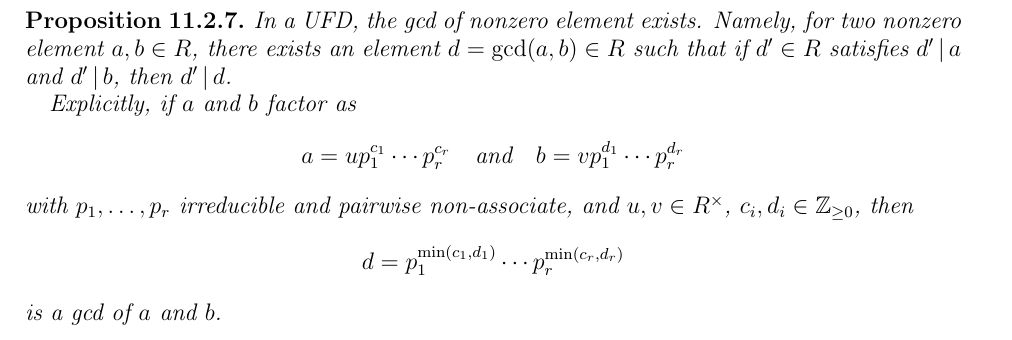
\includegraphics[width=\textwidth]{elementary-ring-theory-2025050920.png}
% \caption{}
\label{}
\end{figure}

\subsubsection{Problem 3}

\begin{exercise}
Suppose that $R$ is a UFD for which every nonzero prime ideal is maximal. Show that $R$ is a PID.
\end{exercise}
\begin{proof}
We first prove that for two prime elements $p$ and $q$, either they are associates, or there exists $a, b \in R$ such that $a p+b q=1$. Indeed, if $p$ and $q$ are not associates, the ideals $(p)$ and $(q)$ cannot have containment relations (otherwise, say $(p) \subseteq(q)$, we must have $q \mid p$; which would immediately forces $p$ and $q$ to be associates). Now as nonzero prime ideals (such as $(p)$ and $(q)$) are maximal, \textbf{the ideal $(p, q)$ must be the unit ideal}, i.e. there exists $a, b \in R$ such that $a p+b q=1$.

Next, we show that if, in the factorization of two elements $c, d \in R$, no prime factors of $c$ are associates of prime factors of $d$, then there exists $a, b \in R$ such that $a c+b d=1$. By induction, it suffices to prove that: if $\left(p_1, q\right)=\left(p_2, q\right)=(1)$, then $\left(p_1 p_2, q\right)=(1)$. Indeed, write $\lambda_1 p_1+\mu_1 q=1$ and $\lambda_2 p_2+\mu_2 q=1$ for $\lambda_1, \lambda_2, \mu_1, \mu_2 \in R$, then
\[
\lambda_1 \lambda_2 p_1 p_2=\left(1-\mu_1 q\right)\left(1-\mu_2 q\right)=1-\left(\mu_1+\mu_2-\mu_1 \mu_2 q\right) q
\]
This implies that $\left(p_1 p_2, q\right)=(1)$.

We finally prove that $R$ is a PID. Let $I$ be a nonzero ideal. Pick an element $x \in I$ with minimal number of prime factors. We show that $I=(x)$. If $y \in I \backslash(x)$, then write $d=\operatorname{gcd}(x, y)$ and $x=d x_d$ and $y=d y_d$ with $x_d, y_d \in R$, and $x_d, y_d$ have distinct prime factors. By the discussion above, there exist $a, b \in R$ such that $a x_d+b y_d=1$. This implies that $d \in I$, contradicting with the minimality of prime factors of $x \in I$. Thus $I$ is a principal ideal.

\end{proof}


\begin{proposition}
PID is Bézout integral domain; UFD may not.
\end{proposition}
\begin{definition}[Bézout domain]
A \textbf{Bézout domain} is an integral domain in which every finitely generated ideal is principal.
\end{definition}
\begin{note}
Equivalently, an integral domain is called Bézout domain provided that for any $a, b\in R$, $\gcd(a,b)\eqqcolon d$ exists, i.e. $(a, b)=(d)$, i.e. $\exists x, y\in R$ s.t.
\[
ax+by=d
\]
\end{note}
By the definition, PID is Bézout domain. But there exists non-Bézout UFD, e.g. $\mathbb{Z}[x]$. Consider $2,x$ in $\mathbb{Z}[x]$; UFD admits gcd; $\gcd(2,x)=1$, but no $p(x),q(x)$ satisfy $2\cdot p(x)+x\cdot q(x)=1$, as letting $x=0$, then $2\cdot p(0)=1$. (a contradiction!)
